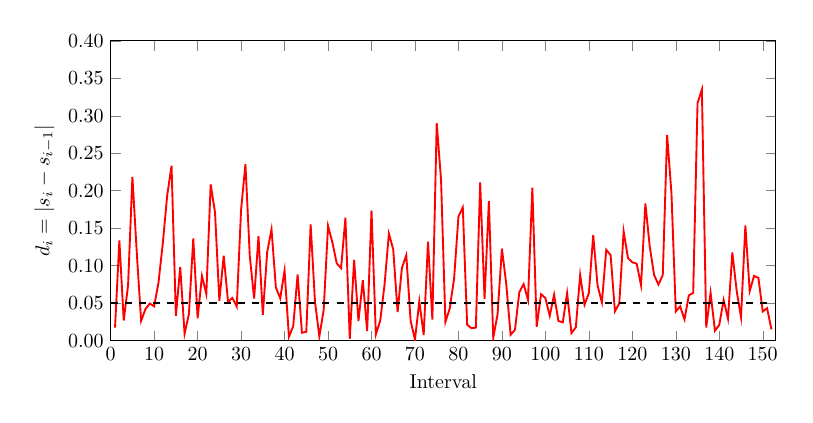
\begin{tikzpicture}[scale=0.85]
\begin{axis}[xmin=0, xmax=153, ymin=0.0, ymax=0.40,
		   width=0.95\textwidth,
		   height=0.50\textwidth,
	 	   x tick label style={scale=0.85,
   		 	/pgf/number format/.cd,
			/pgf/number format/1000 sep={},
   			fixed,
   			fixed zerofill,
    			precision=0
		   },
		   x label style={scale=0.85},
	 	   y tick label style={scale=0.85,
    		 	/pgf/number format/.cd,
   			fixed,
   			fixed zerofill,
    			precision=2
		    },
		   y label style={scale=0.85},
                    xtick={0,10,20,30,40,50,60,70,80,90,100,110,120,130,140,150},
                    ytick={0.0,0.05,0.1,0.15,0.2,0.25,0.3,0.35,0.40},
                    xlabel={Interval},
                    ylabel={$d_i = |s_i-s_{i-1}|$}] 
\addplot[color=red, thick, mark=none] coordinates { 
% 4
(1, 0.01743528402261589)
(2, 0.13373077102878034)%
(3, 0.027012077425515008)
(4, 0.07382808657997819)%
(5, 0.21852390152528353)%
(6, 0.11764203892385178)%
(7, 0.026395340816235097)
(8, 0.04216024487645065)
(9, 0.04964862014065366)
(10, 0.04581763426731142)
% 6
(11, 0.07753883257896926)%
(12, 0.1304020917954295)%
(13, 0.19373103166632877)%
(14, 0.23334303791803462)%
(15, 0.03303768079776079)
(16, 0.09841305033359624)%
(17, 0.009150940625636927)
(18, 0.03577248509165776)
(19, 0.13624939059772012)%
(20, 0.029951726130680978)
% 9
(21, 0.08639503608384025)%
(22, 0.062218906525590756)%
(23, 0.20849932944748895)%
(24, 0.17103383299275118)%
(25, 0.05333658458595614)%
(26, 0.11341634423483318)%
(27, 0.05181274573576222)%
(28, 0.05704167085266157)%
(29, 0.04556098840431605)
(30, 0.17487639384950607)%
% 9
(31, 0.23552697666545755)%
(32, 0.11315591895831131)%
(33, 0.05615323027948087)%
(34, 0.1393708285891777)%
(35, 0.034599656414753335)
(36, 0.11800563249188685)%
(37, 0.14846995323320356)%
(38, 0.07100446568967816)%
(39, 0.05650725911152338)%
(40, 0.09341342947421943)%
% 4
(41, 0.005202811264950036)
(42, 0.019532307681486366)
(43, 0.0883007958591249)%
(44, 0.01056726020784532)
(45, 0.01188745262538049)
(46, 0.15503804357792628)%
(47, 0.051816075553795526)%
(48, 0.005613395759054451)
(49, 0.041040243902571716)
(50, 0.15321145465562896)%
% 7
(51, 0.13109532517470282)%
(52, 0.10317536352552889)%
(53, 0.09664301265379166)%
(54, 0.16399627040217563)%
(55, 0.0025884249419322533)
(56, 0.10772094143320449)%
(57, 0.026311043816498847)
(58, 0.08057134068285793)%
(59, 0.01271577585636624)
(60, 0.17372955589504693)%
% 5
(61, 0.008317418880705016)
(62, 0.026628435316729968)
(63, 0.0747018286856811)%
(64, 0.1428859644621294)%
(65, 0.12161512702065193)%
(66, 0.038056853375573255)
(67, 0.09717530944068783)%
(68, 0.11400648344698563)%
(69, 0.026178298503828135)
(70, 0.0015926282885295184)
% 6
(71, 0.05258017122680689)%
(72, 0.007645548287384368)
(73, 0.13210310485799512)%
(74, 0.02812246544271113)
(75, 0.29006769291940415)%
(76, 0.21435314135509387)%
(77, 0.024970940271326292)
(78, 0.043065797624217)
(79, 0.08302569385865996)%
(80, 0.16555946231472696)%
% 5
(81, 0.1777141106872298)%
(82, 0.021381208065680224)
(83, 0.016639891391438455)
(84, 0.01748048776475164)
(85, 0.21109794116689656)%
(86, 0.055753041202876004)%
(87, 0.1861746180111084)%
(88, 0.003823056422360749)
(89, 0.03519783951807931)
(90, 0.12282565335510365)%
% 7
(91, 0.0753855225126781)%
(92, 0.007848226734326974)
(93, 0.014424796890814162)
(94, 0.06464907696677136)%
(95, 0.07548870363150534)%
(96, 0.054287743986308715)%
(97, 0.20405278965074553)%
(98, 0.01862384980121931)
(99, 0.06207416994675424)%
(100, 0.05686692813089961)%
% 4
(101, 0.03323821140235972)
(102, 0.06131297922012813)%
(103, 0.02622795460016497)
(104, 0.02451482489749246)
(105, 0.06334086256539018)%
(106, 0.010167325045174813)
(107, 0.017831777688085748)
(108, 0.08772996310501494)%
(109, 0.04795885989750573)
(110, 0.06346643762294915)%
% 8
(111, 0.14082901186247046)%
(112, 0.07379897473186192)%
(113, 0.05092561917909336)%
(114, 0.12114730698949988)%
(115, 0.11414816071905845)%
(116, 0.03913382837307944)
(117, 0.04987920442028823)
(118, 0.1456688106253554)%
(119, 0.1100796448759809)%
(120, 0.10455485186493982)%
% 9
(121, 0.1026820801346866)%
(122, 0.0740303777199295)%
(123, 0.18289869559279426)%
(124, 0.1257156866604306)%
(125, 0.08781641623287217)%
(126, 0.07487922132659475)%
(127, 0.08722884612823822)%
(128, 0.27453712431732574)%
(129, 0.19666392968752333)%
(130, 0.0389611229420595)
% 5
(131, 0.04586924521034308)
(132, 0.0283932026951563)
(133, 0.06049424404378906)%
(134, 0.06371828047994896)%
(135, 0.31692322985317745)%
(136, 0.3348924546718697)%
(137, 0.017572925166031678)
(138, 0.06383940073075645)%
(139, 0.013323768703220634)
(140, 0.021013489548163733)
% 6
(141, 0.05438017741655721)%
(142, 0.029440507059259102)
(143, 0.11753537895501415)%
(144, 0.06663596125248478)%
(145, 0.03116904092927375)
(146, 0.15356560064551633)%
(147, 0.06619521231458012)%
(148, 0.08638319875883374)%
(149, 0.08385980146936733)%
(150, 0.03889037855417282)
% 0
(151, 0.04331867359082958)
(152, 0.01506041588130394)
};
\addplot[color=black, thick, dashed] table[row sep = crcr]{0 0.05 \\ 152 0.05 \\};
\end{axis}
\end{tikzpicture}
